%----------------------------------------------------------------------------------------
%
% A LaTeX-template for 1DV510. Modified and translated by Björn Lindenberg at LNU.
% Based on an original master thesis template created by Marcus Wilhelmsson at LNU.
%
%----------------------------------------------------------------------------------------

% Settings and document configuration

\documentclass[a4paper,12pt]{article} 
\usepackage[T1]{fontenc} 
\usepackage{times} 
\usepackage[swedish,english]{babel} 
\usepackage[utf8]{inputenc} 
\usepackage{dtk-logos} 
\usepackage{wallpaper} 
\usepackage[absolute]{textpos} 
\usepackage[top=2cm, bottom=2.5cm, left=3cm, right=3cm]{geometry} 
\usepackage[parfill]{parskip} 
\usepackage{csquotes} 
\usepackage{float} 
\usepackage{lipsum} % Used for dummy text. Can be removed.
\usepackage{listings, color}
\lstdefinestyle{Asm}{
  belowcaptionskip=1\baselineskip,
  breaklines=true,
  frame=L,
  xleftmargin=\parindent,
  language=[x86masm]Assembler,
  showstringspaces=false,
  basicstyle=\footnotesize\ttfamily,
  keywordstyle=\bfseries\color{purple!40!black},
  commentstyle=\itshape\color{green!40!black},
  identifierstyle=\color{blue},
  stringstyle=\color{orange},
}

% Fontsizes for section headings.
\usepackage{sectsty} 
\sectionfont{\fontsize{14}{15}\selectfont}
\subsectionfont{\fontsize{12}{15}\selectfont}
\subsubsectionfont{\fontsize{12}{15}\selectfont}

%----------------------------------------------------------------------------------------
%	This part is used for the text box on the title page
%----------------------------------------------------------------------------------------
\newsavebox{\mybox}
\newlength{\mydepth}
\newlength{\myheight}

\newenvironment{sidebar}%
{\begin{lrbox}{\mybox}\begin{minipage}{\textwidth}}%
{\end{minipage}\end{lrbox}%
 \settodepth{\mydepth}{\usebox{\mybox}}%
 \settoheight{\myheight}{\usebox{\mybox}}%
 \addtolength{\myheight}{\mydepth}%
 \noindent\makebox[0pt]{\hspace{-20pt}\rule[-\mydepth]{1pt}{\myheight}}%
 \usebox{\mybox}}

%----------------------------------------------------------------------------------------
%	Title
%----------------------------------------------------------------------------------------
\newcommand\BackgroundPic{
    \put(-2,-3){
    
\includegraphics[keepaspectratio,scale=0.3]{img/lnu_etch.png} % Background image
    }
}
\newcommand\BackgroundPicLogo{
    \put(30,740){
    
\includegraphics[keepaspectratio,scale=0.10]{img/logo.png} % LNU logo
    }
}

\title{
\vspace{-8cm}
\begin{sidebar}
    \vspace{10cm}
    \normalfont \normalsize
    \huge Computer Technology I\\ % Main title
    \vspace{-1.3cm}
\end{sidebar}
\vspace{3cm}
\begin{flushleft}
    \huge Lab. 4 : Timer and UART % Subtitle
     \small \\ \emph{}
\end{flushleft}
\null
\vfill
\begin{textblock}{5}(10,13)
\begin{flushright}
\begin{minipage}{\textwidth}
\begin{flushleft} \large
\emph{Author:}\textsc{Anas Kwefati}\\  % Author
\emph{Supervisor:}  \textsc{Anders Haggren} \\  % Author
\emph{Semester:} Autumn 2019\\ % Semester
\emph{Area:} Computer Science \\ % Area
\emph{Course code:} 1DT301 % Course
\end{flushleft}
\end{minipage}
\end{flushright}
\end{textblock}
}

\date{} % Empty date command. Use \today inside for today's date.
\author{} % Normally one would use this to define authors. However in this case the title command takes care of everything, so we leave the field empty to get rid of warnings. 

\begin{document}

\pagenumbering{gobble} % Turn off page numbering
\newgeometry{left=5cm}
\AddToShipoutPicture*{\BackgroundPic} % Adds the background image to the title page
\AddToShipoutPicture*{\BackgroundPicLogo} % Adds the logo to the title page
\maketitle % Prints the title
\restoregeometry
\clearpage

\pagenumbering{roman} % Roman page numbering for abstract page


\selectlanguage{english}

\newpage

\pagenumbering{gobble} % Turn off page numbering
\tableofcontents 

\newpage
\pagenumbering{arabic} % Turn on page numbering

%TASK1
\section{Task 1}
\lstset{style=Asm}

\begin{lstlisting}
;>>>>>>>>>>>>>>>>>>>>>>>>>>>>>>>>>>>>>>>>>>>>>>>>>>>>>>>>>>>
; 1DT301, Computer Technology I
; Date: 2016-09-15
; Author:
;	Anas Kwefati
;
; Lab number: 4
; Title: Timer and UART
;
; Hardware: STK600, CPU ATmega2560
;
; Function: Write a program that creates a square wave. The LED has to switch with
; the frequency of 1Hz. Duty cycle 50\%-> ON : 0.5s ; OFF : 0.5s.
; Use Timer interrupt with 2Hz, which change between ON and OFF.
;
; Input ports: None
;
; Output ports: PORTB turns on/off the light (LEDs)
;
; Subroutines: Timer Interrupt Subroutine
; Included files: m2560def.inc
;
; Other information:
;
; Changes in program: (Description and date)
;<<<<<<<<<<<<<<<<<<<<<<<<<<<<<<<<<<<<<<<<<<<<<<<<<<<<<<<<<<<
.include "m2560def.inc"
;The term VECTOR means nothing more than that each interrupt has its specific address where it jumps to.
; The term TABLE means it is a list of jump instructions. This is a list of rjmp or jmp instructions, sorted by interrupt priority


;TCCR0: In this register (used to configure the timer), there are 8 bits, but only last 3 bits CS02,CS01 and CS00 are used.
;These are CLOCK SELECT bits used to setup the prescaler

;TCNT0: This is the real counter in the TIMER0 counter.
;The timer clock counts this register as 1, ie the timer clock increases the value of this 8 bit register by 1 with every timer clock pulse.
; The timer clock can be defined by the TCCRO register

;TIMSK0: This register, used to activate/deactivate the INTERRUPTS related to timers,controls the interrupts of all three timers.
;BIT0 (first bit from the right) controls the the overflow interrupts of TIMER0.
;Note that TIMER0 has one interrupt, and the rest of the bits are for other counters

.org 0x00 ;This is the location that the program will start executing from
rjmp start

;TIMER0 is an 8 bit counter clock
.org OVF0addr
rjmp timer0_int


.org 0x72
start:
	; Initialize SP, Stack Pointer
	ldi r16, HIGH(RAMEND) ; R20 = high part of RAMEND address
	out SPH,r16 ; SPH = high part of RAMEND address
	ldi r16, low(RAMEND) ; R20 = low part of RAMEND address
	out SPL,r16 ; SPL = low part of RAMEND address

	;Main program initialization
	ldi r17, 0xFF ;
	out DDRB, r17 ; we set the DDRB as output

	;TCCR0 control the clock selection
	;This is the to choose the timer to count in ms
	ldi r16, 0b00000101 ;We prescale the value 0x05 = 0b0000 0101 so when we look to TCCR0 table we take clk/1024
	out TCCR0B, r16 ;CS2 - CS2 = 101 osc.clock/1024

	;TIMSK or Timer Interrupt Mask Register allows to set TOIEx and 1bit in SREG to enable overflow interrupt
	ldi r16, 0b00000001 ;we choose 0000 0001 Timer0 ;TOIE0 Timer Overflow Interrupt Enable (TIMER0)
	sts TIMSK0, r16  ;We output it in register TIMSK


	ldi r16, 155 ;Starting value for counter it counts from 155 to 255
	;So it will take 100ms to go from 155 to 255.
	out TCNT0, r16 ;We output the counter in Register TCNT0 (Real counter in the TIMER0)

	ldi r19, 0b00000000 ;TO turn on the light

	sei ;enabling all interrupts


main_program:
nop
rjmp main_program

ldi r17, 0 ;COUNTER

timer0_int :
	;Important to not do multiple interrupts at the same time and do one by one
	push r16 ;timer interrupt routine
	in r16, SREG ;save SREG on stack
	push r16

	;WE SET THE COUNTER TCNT0 back
	ldi r16, 155
	out TCNT0, r16


	inc r17 ;increase r17

	cpi r17,5   ;compare r17 with how many time it goes inside this interrupt
	;we take 5, because 5x100ms = 500ms so it will be the half of 1000ms
	brne continue

	ldi r17, 0 ;reset r17 the counter

	com r19 ;complement of r19 to turn off the light
	out PORTB, r19 ;Output r19 to PORTB

	continue :
		nop

	;It allows to exit the interrupt by restoring SREG
	pop r16 ;restore SREG
	out SREG, r16
	pop r16 ;restore register


RETI ;return from interrupt

\end{lstlisting}


\begin{figure}
\begin{center}
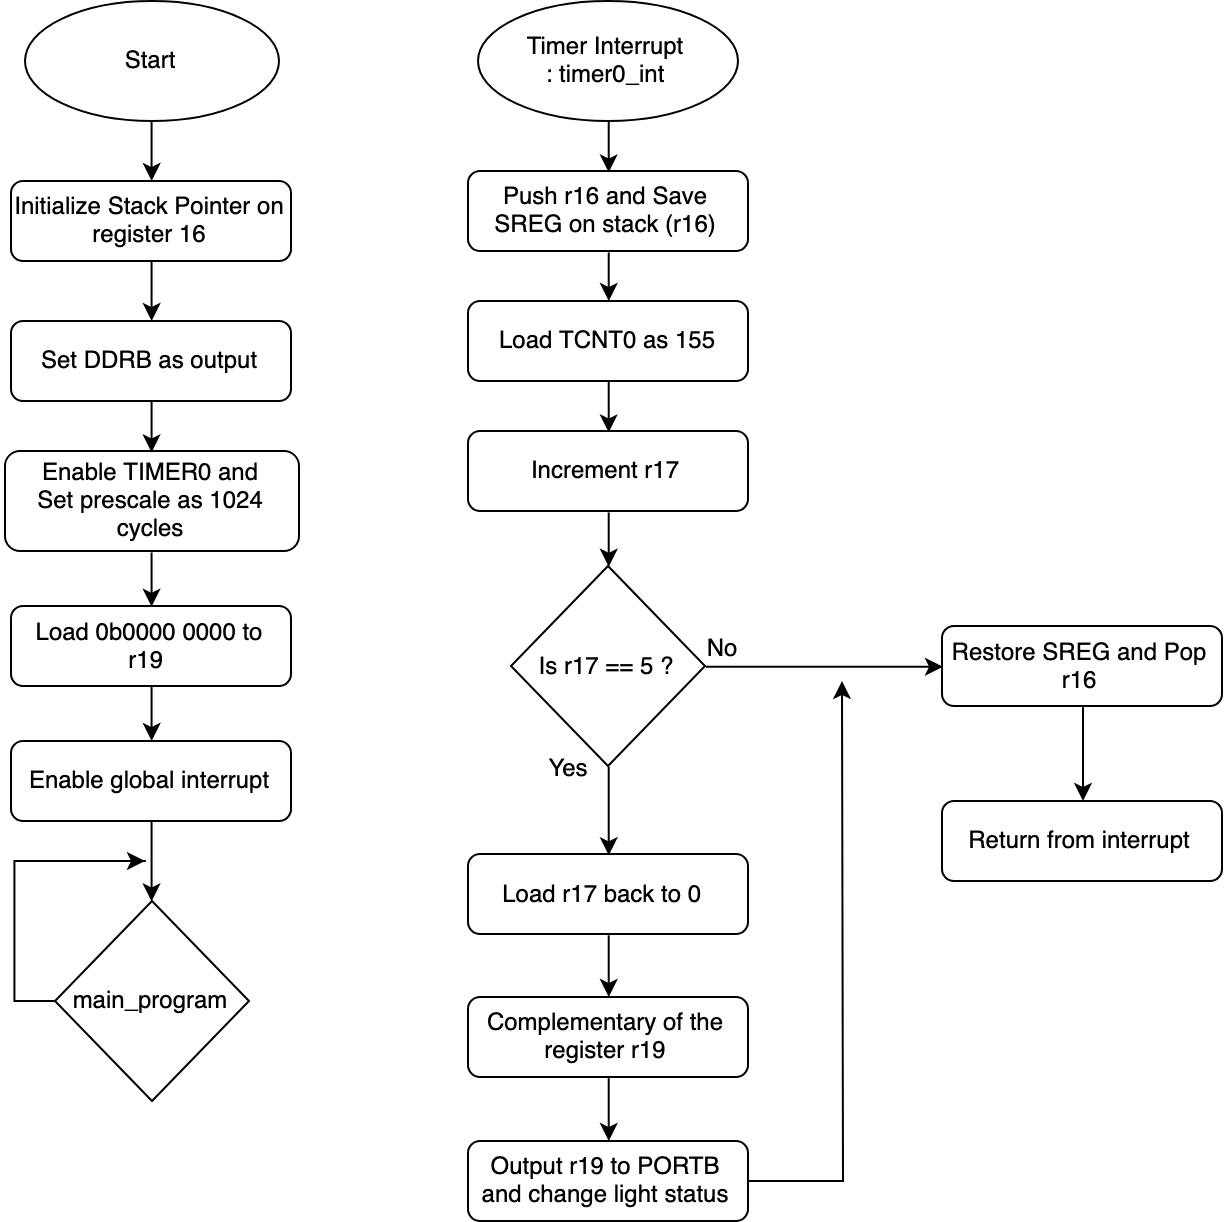
\includegraphics[width=\textwidth/1 ]{flowchart/task1_flowchart.png}
\end{center}
\caption{Task 1 flowchart}
\label{task1}
\end{figure}
\break


%TASK2
\section{Task 2}

\lstset{style=Asm}

\begin{lstlisting}
;>>>>>>>>>>>>>>>>>>>>>>>>>>>>>>>>>>>>>>>>>>>>>>>>>>>>>>>>>>>
; 1DT301, Computer Technology I
; Date: 2016-09-15
; Author:
;	Anas Kwefati
;
; Lab number: 4
; Title: Timer and UART
;
; Hardware: STK600, CPU ATmega2560
;
; Function: Change TASK 1 program to get Pulse Width Modulation (PWM).
; Frequency should be fixed but the Duty Cycle should be able to change.
; Use 2 push buttons to change the duty cycle up and down.
; Duty Cycle should be able to change from 0\% to 100\% in steps of 5\%.
;
; Input ports: PORTD to press buttons SW0 and SW1.
;
; Output ports: PORTB turns on/off the light (LEDs)
;
; Subroutines: Timer Interrupt Subroutine
; Included files: m2560def.inc
;
; Other information:
;
; Changes in program: (Description and date)
;<<<<<<<<<<<<<<<<<<<<<<<<<<<<<<<<<<<<<<<<<<<<<<<<<<<<<<<<<<<
.include "m2560def.inc"
;The term VECTOR means nothing more than that each interrupt has its specific address where it jumps to.
; The term TABLE means it is a list of jump instructions. This is a list of rjmp or jmp instructions, sorted by interrupt priority


.org 0x00 ;This is the location that the program will start executing from
rjmp start

;TIMER0 is an 8 bit counter clock
.org OVF0addr
rjmp timer0_int

.org INT0addr
rjmp up

.org INT1addr
rjmp down


.org 0x72
start:
	; Initialize SP, Stack Pointer
	ldi r16, HIGH(RAMEND) ; R20 = high part of RAMEND address
	out SPH,r16 ; SPH = high part of RAMEND address
	ldi r16, low(RAMEND) ; R20 = low part of RAMEND address
	out SPL,r16 ; SPL = low part of RAMEND address

	;Main program initialization
	ldi r17, 0xFF ;
	out DDRB, r17 ; we set the DDRB as output


	ldi r17, 0x00
	out DDRD, r17 ; We set DDRD as input

	out PORTB, r17 ; Turn off all LEDs


	;INTERRUPT INITIALIZATION


	ldi r22, 0b00000011 ;we set the corresponding bit number to enable the related interrupt here INT0
	out EIMSK, r22 ; Toggle external interrupt requests


	ldi r22, 0b00001010 ;We define the type of signals that activates the external interrupt , here we set it as falling edge to activate the interrupt
	sts EICRA, r22 ;we configure when to switch the external interrupt




	;TIMER INITIALIZATION

	;TCCR0 control the clock selection
	;This is the to choose the timer to count in ms
	ldi r16, 0b00000101 ;We prescale the value 0x05 = 0b0000 0101 so when we look to TCCR0 table we take clk/1024
	out TCCR0B, r16 ;CS2 - CS2 = 101 osc.clock/1024

	;TIMSK or Timer Interrupt Mask Register allows to set TOIEx and 1bit in SREG to enable overflow interrupt
	ldi r16, 0b00000001 ;we choose 0000 0001 Timer0 ;TOIE0 Timer Overflow Interrupt Enable (TIMER0)
	sts TIMSK0, r16  ;We output it in register TIMSK

	ldi r16, 205 ;Starting value for counter it counts from 205 to 255, so it will take 50ms ;
	out TCNT0, r16 ;We output the counter in Register TCNT0 (Real counter in the TIMER0)



	;SIMPLE CONFIGURATION

	ldi r19, 0b00000000 ;TO turn on the light

	ldi r21, 10 ; DUTY CYCLE COUNTER we put 10 because it is half of 20 so 50\%
	;20 ETAPE MAX CHAQUE ETAPE PREND 50MS

	ldi r17, 0 ;COUNTER

	sei ;enabling all interrupts


main_program:
nop
rjmp main_program

timer0_int :

	;Important to not do multiple interrupts at the same time and do one by one
	;We enter the timer interrupt instruction
	push r16 ;timer interrupt routine
	in r16, SREG ;save SREG on stack
	push r16

	;WE SET THE COUNTER TCNT0 back
	ldi r16, 205
	out TCNT0, r16

	inc r17 ;increase r17

	cpi r17, 20
	breq reset



	cp r17, r21  ;compare r17 with how many time it goes inside
	brlt turn_on



	turn_off :
		ldi r19,0xFF ;complement of r19 to turn off the light
		out PORTB, r19 ;Output r19 to PORTB
		rjmp end

	turn_on :
		ldi r19, 0b00000000 ;TO turn on the light
		out PORTB, r19 ;Output r19 to PORTB
		rjmp end

	reset :
		ldi r17, 0 ;COUNTER


	end :
	;We exit the timer interrupt instruction
	pop r16 ;restore SREG
	out SREG, r16
	pop r16 ;restore register


RETI ;return from interrupt


up :
	cpi r21, 20 ;we put 20 because 100/5 = 20 hence we need 5 times 20 to reach 100 which is 100 so we count till 20
	brne increase
	increase :
		inc r21
RETI

down :
	cpi r21, 0 ;we put 20 because 100/5 = 20 hence we need 5 times 20 to reach 100 which is 100 so we count till 20
	brne decrease
	decrease :
		dec r21
RETI

;So, we decided to put TCNT0 to 205, like that it will take 50ms to reach 255
;We decided to put 205 because we want to match the duty and the counters
; like that they both go from 0 to 20. 20 was found because we know that the duty goes from 0 to 100\% with a step of 5\%
;If we do 100/5 we get 20. So we need 20 maximum step to reach 100\%.
;1000ms/50ms = 20 steps
;The duty counter starts at 10, because the duty cycle has to be at 50\%.
;So we take the half step of 20 which is 10.
;Hence we compare the counter with the duty.

\end{lstlisting}

\begin{figure}
\begin{center}
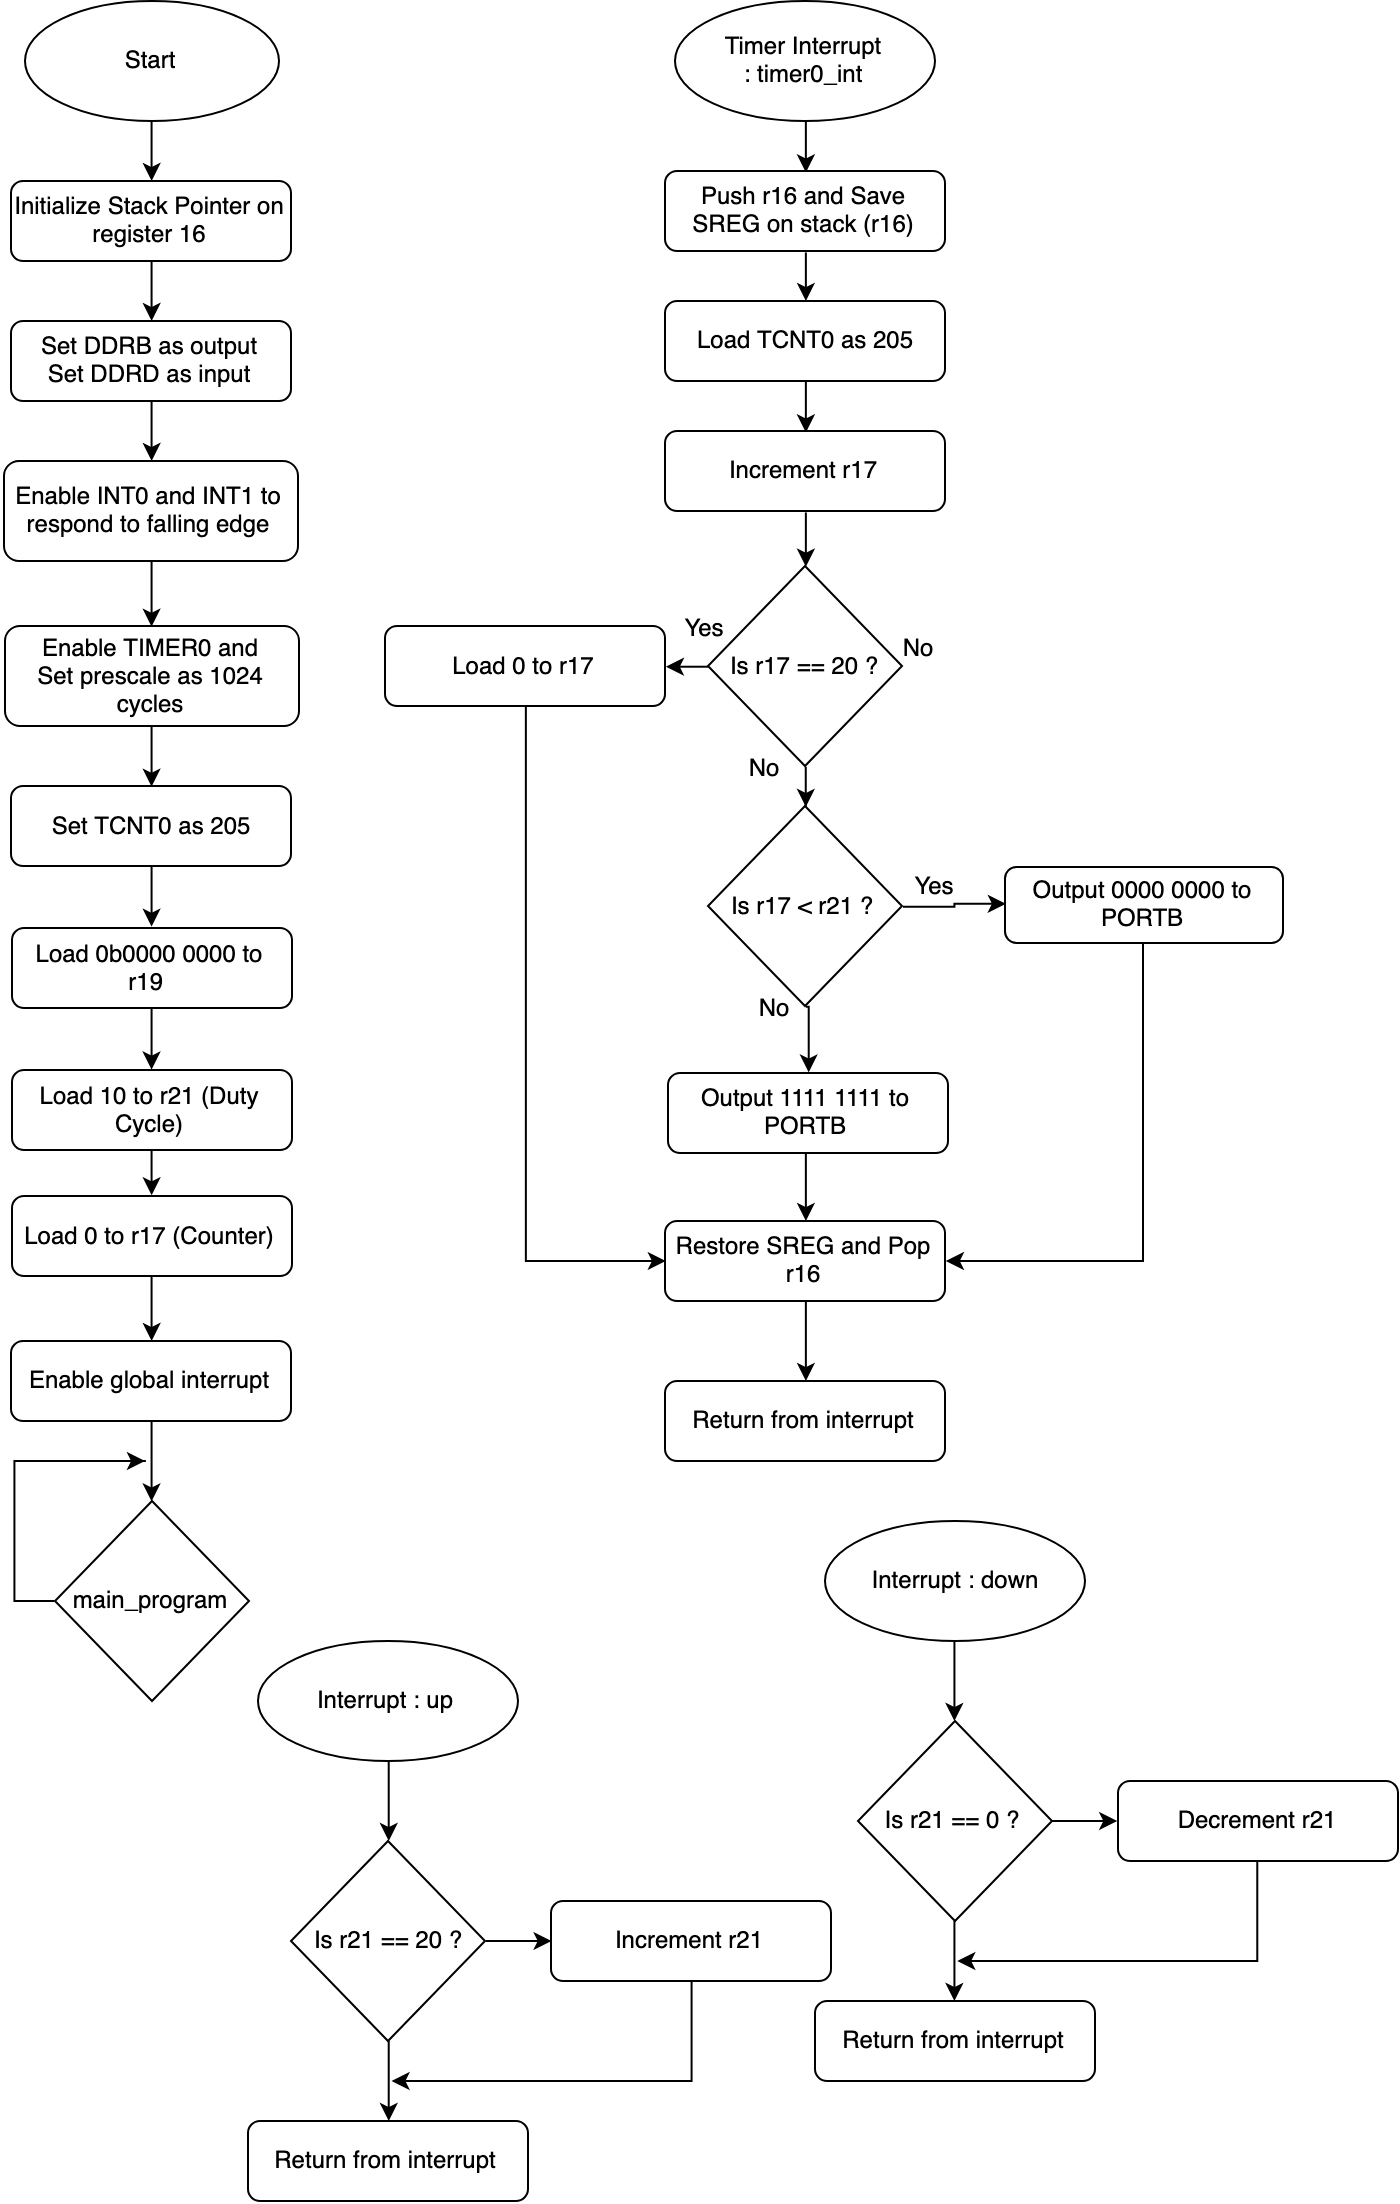
\includegraphics[width=\textwidth/1]{flowchart/task2_flowchart.png}
\end{center}
\caption{Task 2 flowchart}
\label{task2}
\end{figure}




%TASK 3
\break
\section{Task 3}

\lstset{style=Asm}

\begin{lstlisting}
;>>>>>>>>>>>>>>>>>>>>>>>>>>>>>>>>>>>>>>>>>>>>>>>>>>>>>>>>>>>
; 1DT301, Computer Technology I
; Date: 2016-09-15
; Author:
;	Anas Kwefati
;
; Lab number: 4
; Title: Timer and UART
;
; Hardware: STK600, CPU ATmega2560
;
; Function: Program that uses the serial communication PORT0 (RS232).
;The program should receive characters that are sent from the computer and show the code on the LEDs.
;
; Input ports: PORT0 (RS232) VGA
;
; Output ports: PORTB turns on/off the light (LEDs)
;
; Subroutines: Timer Interrupt Subroutine
; Included files: m2560def.inc
;
; Other information:
;The code for this exercice was taken from the lecture.
; Changes in program: (Description and date)
;<<<<<<<<<<<<<<<<<<<<<<<<<<<<<<<<<<<<<<<<<<<<<<<<<<<<<<<<<<<
.include "m2560def.inc"

.org 0x00
rjmp start

.org 0x72

start:	;To initialize everything
	ldi r16,0xFF	;PORTB outputs
	out DDRB, r16

	out PORTB,r16	;Iniatial value to outputs

	ldi r16, 12	;osc = 1MHz, 4800 bps => UBBRR = 12
	sts UBRR1L , r16	;Store Prescaler value in UBRR1L

	ldi r16, (1<<RXEN1)	;Set RX enable flags
	sts UCSR1B, r16

GetChar:	;Receive data
	lds r16, UCSR1A	;read UCSR1A I/0 register to r16
	sbrs r16,RXC1	;RXC1=1 -> new Character Skip if bit RXC1 is set in r16
	rjmp GetChar	;RXC1=0 -> no character received otherwise rjmp
	lds r18,UDR1	;Read character in UDR

Port_output:	;Show data on the LEDs
	com r18	;COM to have the 1s become 0s as asked for the exercice
	out PORTB,r18	;Write character to PORTB
	com r18	;COM again to make it normal

\end{lstlisting}

\begin{figure}
\begin{center}
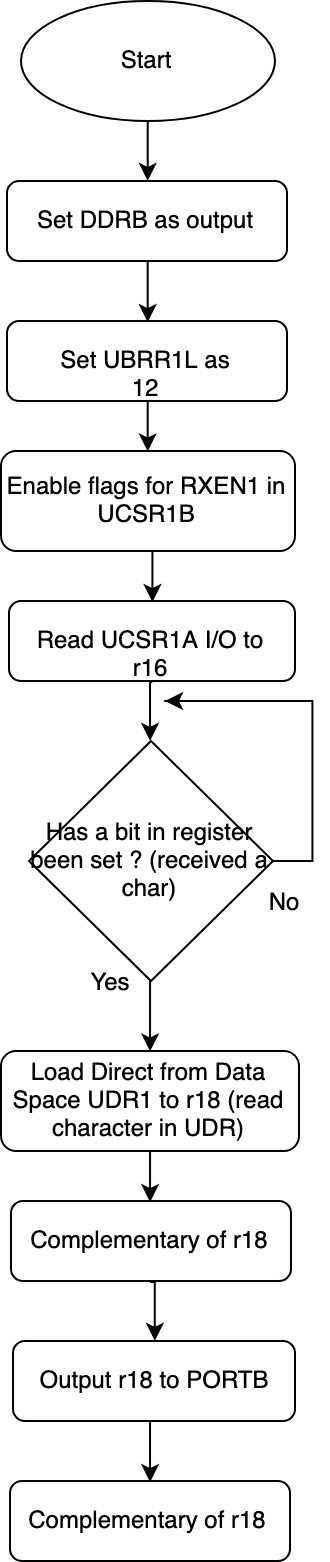
\includegraphics[width=\textwidth/3 ]{flowchart/task3_flowchart.png}
\end{center}
\caption{Task 3 flowchart}
\label{task3}
\end{figure}

\break

%TASK4
\section{Task 4}

\lstset{style=Asm}

\begin{lstlisting}
;>>>>>>>>>>>>>>>>>>>>>>>>>>>>>>>>>>>>>>>>>>>>>>>>>>>>>>>>>>>
; 1DT301, Computer Technology I
; Date: 2016-09-15
; Author:
;	Anas Kwefati
;
; Lab number: 4
; Title: Timer and UART
;
; Hardware: STK600, CPU ATmega2560
;
; Function: Modify task 3 to obtain an echo. The program should receive the character
;and send it back to the terminal. 
;
; Input ports: PORT0 (RS232) VGA
;
; Output ports: PORTB turns on/off the light (LEDs)
;
; Subroutines: Timer Interrupt Subroutine
; Included files: m2560def.inc
;
; Other information:
;The code for this exercice was taken from the lecture.
; Changes in program: (Description and date)
;<<<<<<<<<<<<<<<<<<<<<<<<<<<<<<<<<<<<<<<<<<<<<<<<<<<<<<<<<<<
.include "m2560def.inc"

.org 0x00
rjmp start

.org 0x72


start:
	ldi r16,0xFF	;Set PORTB as output
	out DDRB, r16

	out PORTB,r16	;Iniatialize LEDs state

	ldi r16, 12		;osc = 1MHz, 4800 bps => UBBRR = 12
	sts UBRR1L , r16	;Store Prescaler value in UBRR1L

	ldi r16, (1<<RXEN1 | 1<<TXEN1);Set RX and TX enable flags
	sts UCSR1B, r16

GetChar:	;Receive data
	lds r16, UCSR1A	;read UCSR1A I/0 register to r16
	sbrs r16,RXC1	;RXC1=1 -> new Character
	rjmp GetChar	;RXC1=0 -> no character received
	lds r18,UDR1	;Read character in UDR

Port_output:	;Show Data on LEDs
	com r18
	out PORTB,r18	;Write character to PORTB
	com r18

PutChar:	;Show data back to the terminal
	lds r16, UCSR1A	;Read UCSR1A i/O register to r16
	sbrs r16, UDRE1	;UDRE1 =1 => buffer is empty
	rjmp PutChar	;UDRE1 = 0 => buffer is not empty
	sts UDR1,r18	;write character to UDR1
	rjmp GetChar	;Return to loop

\end{lstlisting}

\begin{figure}
\begin{center}
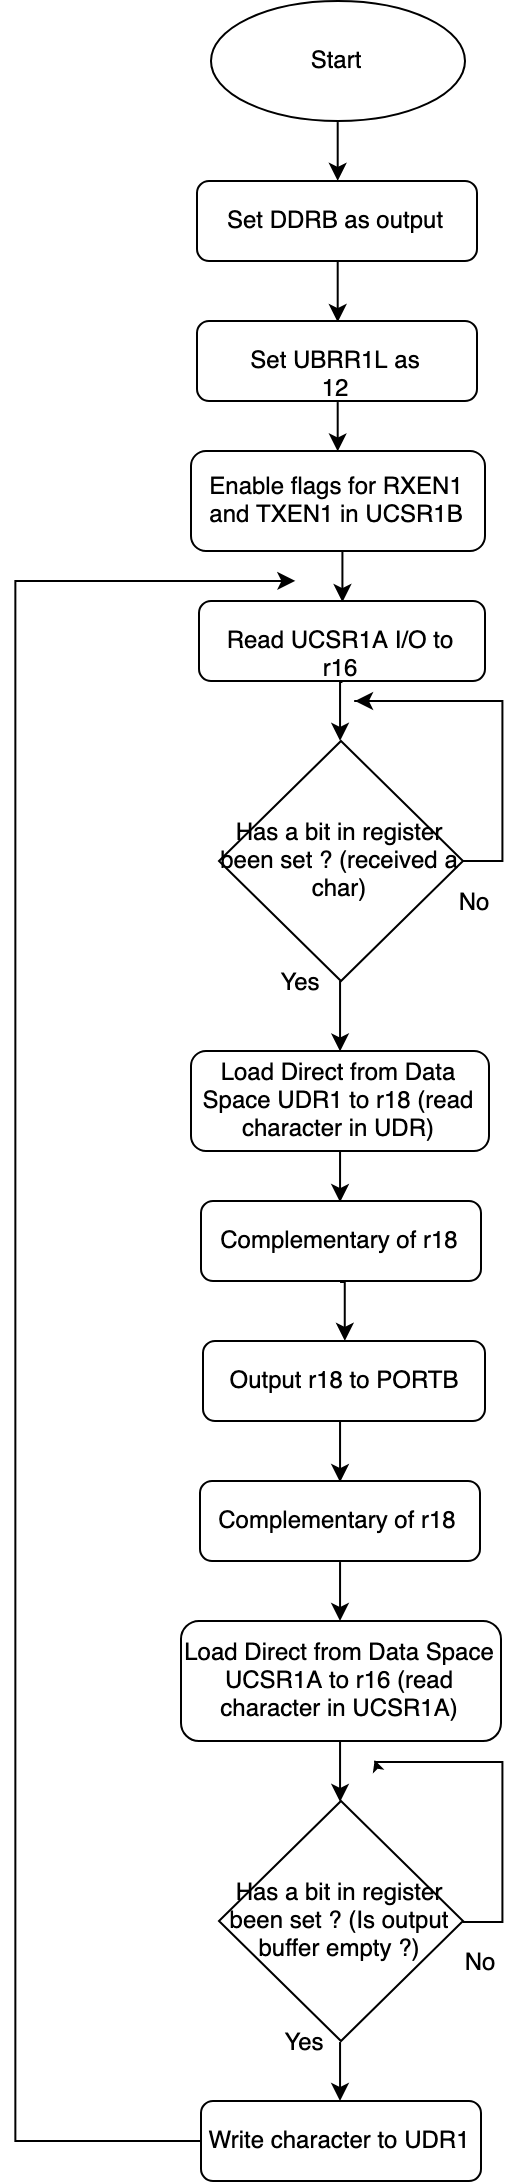
\includegraphics[width=\textwidth/3 ]{flowchart/task4_flowchart.png}
\end{center}
\caption{Task 4 flowchart}
\label{task4}
\end{figure}

\break

%TASK5
\section{Task 5}

\lstset{style=Asm}

\begin{lstlisting}
;>>>>>>>>>>>>>>>>>>>>>>>>>>>>>>>>>>>>>>>>>>>>>>>>>>>>>>>>>>>
; 1DT301, Computer Technology I
; Date: 2016-09-15
; Author:
;	Anas Kwefati
;
; Lab number: 4
; Title: Timer and UART
;
; Hardware: STK600, CPU ATmega2560
;
; Function: Do task 3 and 4 but using Interrupt instead of polled UART.
;
; Input ports: PORT0 (RS232) VGA
;
; Output ports: PORTB turns on/off the light (LEDs)
;
; Subroutines: Timer Interrupt Subroutine
; Included files: m2560def.inc
;
; Other information:
;The code for this exercice was taken from the lecture.
; Changes in program: (Description and date)
;<<<<<<<<<<<<<<<<<<<<<<<<<<<<<<<<<<<<<<<<<<<<<<<<<<<<<<<<<<<
.include "m2560def.inc"

.org 0x00
rjmp start

.org URXC1addr	;USART Interrupt
rjmp GetChar

.org 0x72


start:
	ldi r16,LOW(RAMEND)	;iniatilize SP
	out SPL,r16
	ldi r16,HIGH(RAMEND)
	out SPH,r16

	ldi r16,0xFF	;Set PORTB as output
	out DDRB, r16
	out PORTB,r16	;Initialize LEDs



	ldi r16, 12		;osc = 1MHz, 4800 bps => UBBRR = 12
	sts UBRR1L , r16	;Store Prescaler value in UBRR1L

	ldi r16, 0b10011000;Set RX, TX enable flags and RXCIE = 1
	sts UCSR1B, r16

	sei	;Set global interrupt flag

main_program:
nop		;Infinite loop that does nothing
rjmp main_program

GetChar:	;Receive data
	lds r16, UCSR1A	;read UCSR1A I/0 register to r16
	lds r18,UDR1	;Read character in UDR

  Port_output:	;Show data on the LEDs
  	com r18
  	out PORTB,r18	;Write character to PORTB
  	com r18

  PutChar:	;Sends back the character to the Terminal
  	lds r16, UCSR1A	;Read UCSR1A i/O register to r16
  	sts UDR1,r18	;write character to UDR1

RETI	;Return from interrupt

\end{lstlisting}

\break
\begin{figure}
\begin{center}
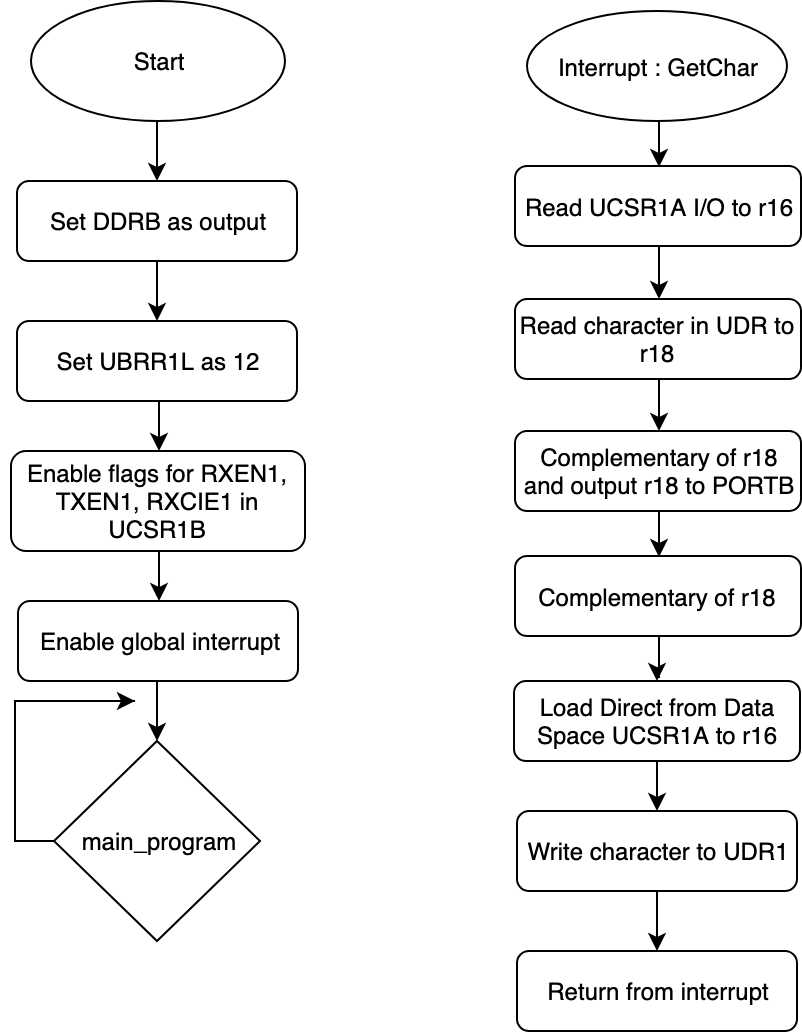
\includegraphics[width=\textwidth/2 ]{flowchart/task5_flowchart.png}
\end{center}
\caption{Task 4 flowchart}
\label{task4}
\end{figure}

\break 

% Prints your bibliography database xxx.bib
\bibliographystyle{IEEEtran}
\bibliography{ref.bib}

\end{document}
